\documentclass[a4paper]{article}

\usepackage[UTF8]{ctex}
\usepackage[a4paper,margin=1in]{geometry}
\usepackage{graphicx}
\usepackage{float}
\usepackage{listings}
\usepackage{longtable}
\usepackage{booktabs}
\usepackage{hyperref}
\usepackage{fancyhdr}
\usepackage{lastpage}
\usepackage{color}
\usepackage{indentfirst}        % 首段缩进
\setlength{\parindent}{2em}     % 缩进2字符
\usepackage{zhnumber}           % 中文编号
\usepackage[dvipsnames]{xcolor}

%\newcommand{\college}{中山大学计算机学院}
\newcommand{\projname}{数据库系统原理实验| 实验1}
\newcommand{\reporttitle}{数据库系统原理实验一}
\newcommand{\stuno}{23336179}
\newcommand{\authorname}{马福泉}
\newcommand{\major}{计算机科学与技术}
\newcommand{\adviser}{赖韩江}
\newcommand{\startdate}{2025年9月18日}
\newcommand{\labenddate}{2025年9月18日}
\newcommand{\labroom}{B202}

\pagestyle{fancy} % 使用 fancyhdr 风格
\fancyhf{}      % 清空默认的页眉页脚

% 设置页眉
\fancyhead[L]{\kaishu \projname}      % 左侧页眉显示项目名称
\fancyhead[C]{\kaishu \reporttitle}    % 中间页眉显示报告标题
\fancyhead[R]{\kaishu \authorname} % 右侧页眉显示作者姓名

% 设置页脚
\fancyfoot[C]{第 \thepage 页，共 \pageref{LastPage} 页} % 中间页脚显示页码

% 去除页眉页脚与正文之间的分隔线
\renewcommand{\headrulewidth}{0.4pt}
\renewcommand{\footrulewidth}{0pt}

% 设置文档背景颜色
\definecolor{mybgcolor}{RGB}{0, 0, 0} % 定义背景颜色
\definecolor{NavyBlue}{RGB}{0,0,128} % 添加颜色定义
% \pagecolor{mybgcolor} % 设置背景颜色

% listing 配置rust
% \lstdefinelanguage{Rust}{
%   keywords={fn, let, mut, struct, enum, impl, pub, use, mod, trait, where},
%   keywordstyle=\color{NavyBlue},
%   comment=[l]{//},
%   commentstyle=\color{gray},
% }
% \lstset{language=Rust}

\begin{document}

% 封面
\begin{titlepage}
    \centering
    

    
\includegraphics[width=10cm]{img/SYSULogo.png}

    \vspace{1em}
    %{\Large \college \par}
    \vspace{1em}
    {\Large \kaishu \projname \par}
    \vspace{3em}

    

    
    {\fontsize{40pt}{42pt}\kaishu \selectfont \boldmath \reporttitle\par}
    \vspace*{\fill}

    \begin{center}
    {\Large
    \makebox[5em][s]{学号}:\underline{\makebox[15em][c]{\kaishu \stuno}}\\[1em]
    \makebox[5em][s]{姓名}:\underline{\makebox[15em][c]{\kaishu \authorname}}\\[1em]
    \makebox[5em][s]{专业}:\underline{\makebox[15em][c]{\kaishu \major}}\\[1em]
    \makebox[5em][s]{指导教师}:\underline{\makebox[15em][c]{\kaishu \adviser}}\\[1em]
    \makebox[5em][s]{起始日期}:\underline{\makebox[15em][c]{\kaishu \startdate}}\\[1em]
    \makebox[5em][s]{结束日期}:\underline{\makebox[15em][c]{\kaishu \labenddate}}\\[1em]
    \makebox[5em][s]{实验地点}:\underline{\makebox[15em][c]{\kaishu \labroom}}
    }
    \end{center}

    \vspace*{\fill}
\end{titlepage}

% 目录
\tableofcontents
\newpage

\section{实验概述}

\subsection{实验目的}

\begin{enumerate}
    \item 理解和掌握数据库DDL语言，能够熟悉地使用SQL DDL语句创建、修改和删除数据库和表。
\end{enumerate}

\subsection{实验内容}

\begin{enumerate}
    \item 使用SQL Server Management Studio创建图书借阅数据库JY。
    \item 按照“图书借阅数据库系统”的设计要求，对下列三张表进行详细设计，并用SQL语言创建：
    
    \begin{enumerate}
        \item 图书表 book：
        
        \begin{table}[H]
        \centering
        \begin{tabular}{llll}
        \toprule
        列名 & 说明 & 数据类型 & 列的约束 \\
        \midrule
        book\_id & 图书编号 & char(8) & NOT NULL \\
        book\_name & 书名 & nvarchar(50) & NOT NULL \\
        book\_isbn & 图书isbn号 & char(17) & NOT NULL \\
        book\_author & 作者 & nvarchar(10) & NOT NULL \\
        book\_publisher & 出版社 & nvarchar(50) & NOT NULL \\
        book\_price & 价格 & money & NOT NULL \\
        interview\_times & 借阅次数 & smallint & NOT NULL \\
        \bottomrule
        \end{tabular}
        \caption{图书表 book}
        \end{table}

        \item 读者表 reader：
        
        \begin{table}[H]
        \centering
        \begin{tabular}{llll}
        \toprule
        列名 & 说明 & 数据类型 & 列的约束 \\
        \midrule
        reader\_id & 读者编号 & char(8) & NOT NULL \\
        reader\_name & 姓名 & nvarchar(50) & NOT NULL \\
        reader\_sex & 性别 & char(2) & NOT NULL \\
        reader\_department & 院系 & nvarchar(60) & NOT NULL \\
        \bottomrule
        \end{tabular}
        \caption{读者表 reader}
        \end{table}

        \item 借阅记录表 record：
        
        \begin{table}[H]
        \centering
        \begin{tabular}{llll}
        \toprule
        列名 & 说明 & 数据类型 & 列的约束 \\
        \midrule
        reader\_id & 读者编号 & char(8) & NOT NULL \\
        book\_id & 图书编号 & char(8) & NOT NULL \\
        borrow\_date & 借书时间 & date & NOT NULL \\
        return\_date & 还书时间 & date & NOT NULL \\
        notes & 备注 & nvarchar(50) & NOT NULL \\
        \bottomrule
        \end{tabular}
        \caption{借阅记录表 record}
        \end{table}
    \end{enumerate}

    \item 使用ALTER TABLE语句对book表进行如下操作：
    \begin{enumerate}
        \item 在图书表book中插入新列 total，数据类型是smallint，NOT NULL；
        \item 在图书表book中修改interview\_times列的数据类型为int；
        \item 在图书表book中删除total列。
    \end{enumerate}
\end{enumerate}

\section{实验报告}

\subsection{1. 创建数据库JY}

本实验首先在SQL Server Management Studio中创建数据库JY。

\begin{lstlisting}[language=SQL]
CREATE DATABASE JY;
GO
\end{lstlisting}

\begin{figure}[H]
    \centering
    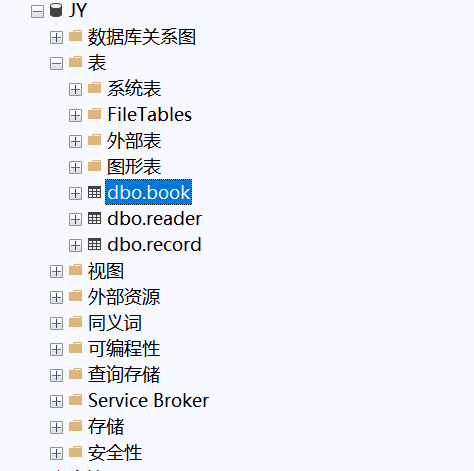
\includegraphics[width=0.7\textwidth]{img/create_db.png}
    \caption{创建数据库JY结果}
\end{figure}

\subsection{2. 创建数据表}

根据设计要求，分别创建图书表book、读者表reader、借阅记录表record。

% SQL脚本代码照片
\begin{figure}[H]
    \centering
    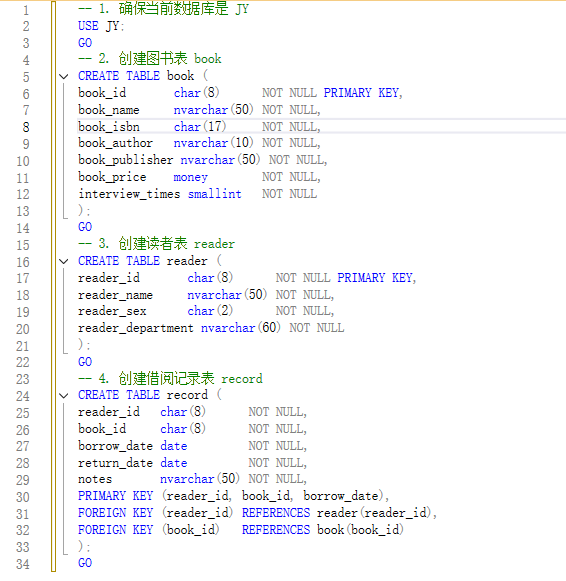
\includegraphics[width=0.85\textwidth]{img/script.png}
    \caption{创建三张数据表的SQL脚本}
\end{figure}

% 数据库关系图
\begin{figure}[H]
    \centering
    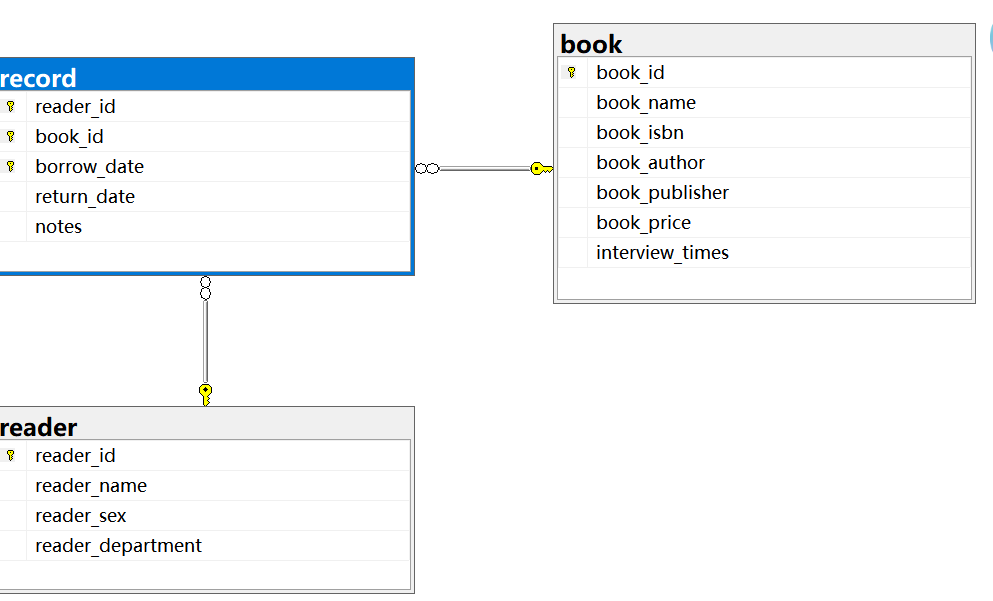
\includegraphics[width=0.85\textwidth]{img/structure.png}
    \caption{图书借阅数据库关系结构图}
\end{figure}

\subsubsection{2.1 创建图书表book}

% 代码展示区
\begin{lstlisting}[language=SQL]
CREATE TABLE book (
    book_id char(8) NOT NULL,
    book_name nvarchar(50) NOT NULL,
    book_isbn char(17) NOT NULL,
    book_author nvarchar(10) NOT NULL,
    book_publisher nvarchar(50) NOT NULL,
    book_price money NOT NULL,
    interview_times smallint NOT NULL
);
\end{lstlisting}

\begin{figure}[H]
    \centering
    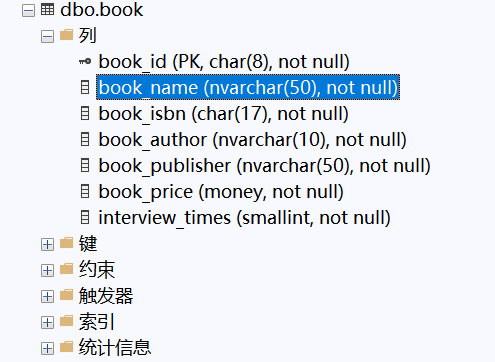
\includegraphics[width=0.7\textwidth]{img/create_book.png}
    \caption{创建book表结果}
\end{figure}

\subsubsection{2.2 创建读者表reader}

% 代码展示区
\begin{lstlisting}[language=SQL]
CREATE TABLE reader (
    reader_id char(8) NOT NULL,
    reader_name nvarchar(50) NOT NULL,
    reader_sex char(2) NOT NULL,
    reader_department nvarchar(60) NOT NULL
);
\end{lstlisting}

\begin{figure}[H]
    \centering
    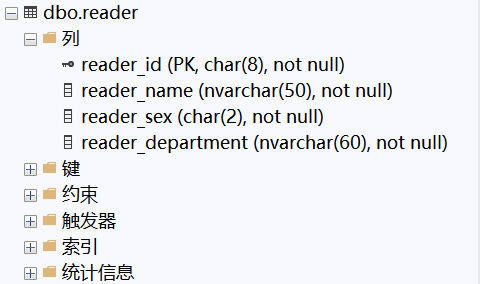
\includegraphics[width=0.7\textwidth]{img/create_reader.png}
    \caption{创建reader表结果}
\end{figure}

\subsubsection{2.3 创建借阅记录表record}

% 代码展示区
\begin{lstlisting}[language=SQL]
CREATE TABLE record (
    reader_id char(8) NOT NULL,
    book_id char(8) NOT NULL,
    borrow_date date NOT NULL,
    return_date date NOT NULL,
    notes nvarchar(50) NOT NULL
);
\end{lstlisting}

\begin{figure}[H]
    \centering
    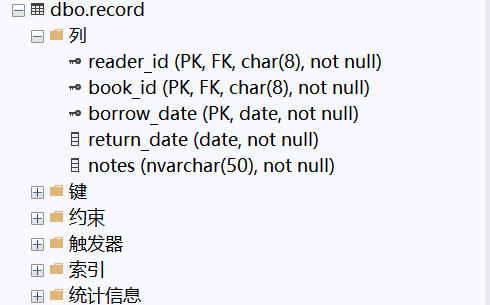
\includegraphics[width=0.7\textwidth]{img/create_record.png}
    \caption{创建record表结果}
\end{figure}

% 添加说明注释的SQL代码截图
\begin{figure}[H]
    \centering
    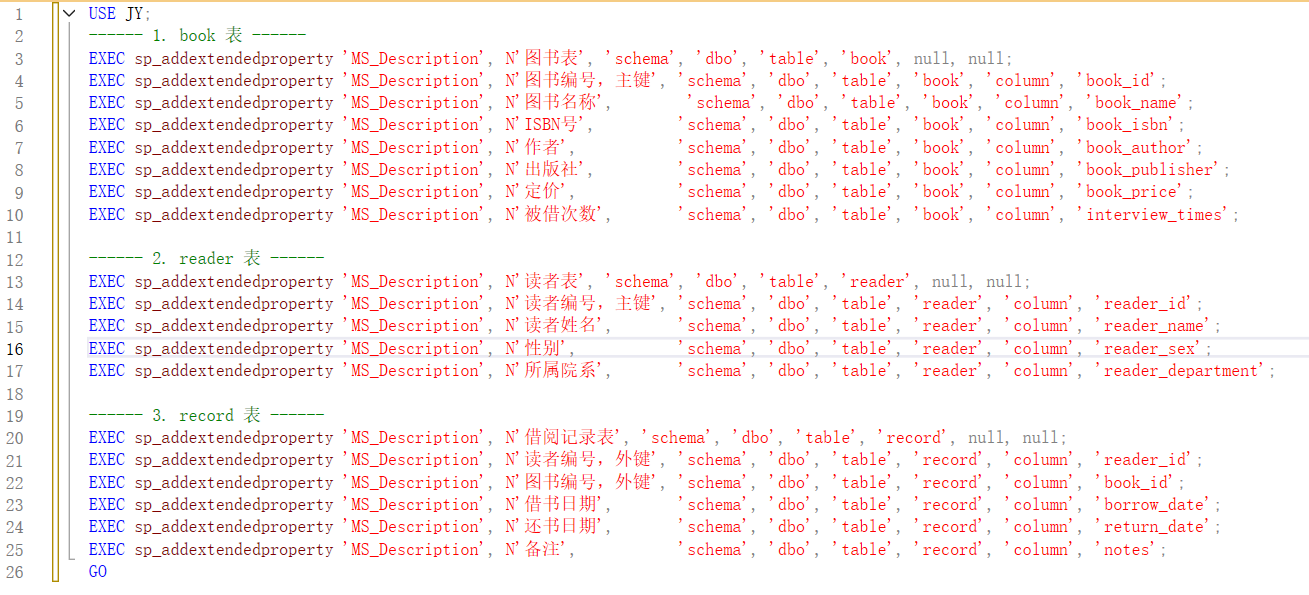
\includegraphics[width=1.0\textwidth]{img/add_annotion.png}
    \caption{为三张表添加说明注释的SQL代码截图}
\end{figure}

% 结果截图
\begin{figure}[H]
    \centering
    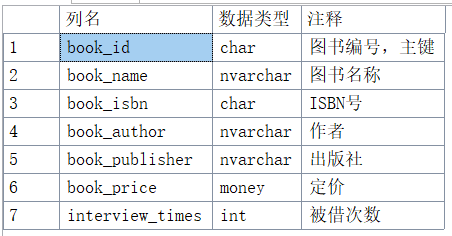
\includegraphics[width=0.7\textwidth]{img/book_annotation.png}
    \caption{book表添加注释结果}
\end{figure}

\begin{figure}[H]
    \centering
    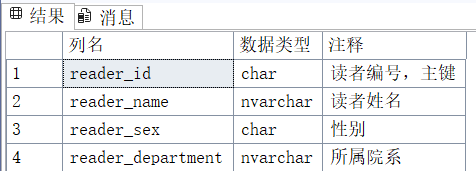
\includegraphics[width=0.7\textwidth]{img/reader_annotation.png}
    \caption{reader表添加注释结果}
\end{figure}

\begin{figure}[H]
    \centering
    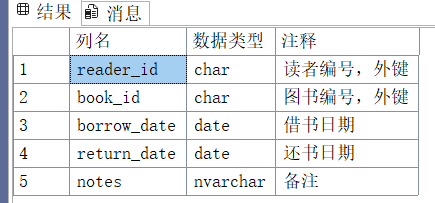
\includegraphics[width=0.7\textwidth]{img/record_annotation.png}
    \caption{record表添加注释结果}
\end{figure}

\subsection{3. 使用ALTER TABLE语句修改数据表}

\subsubsection{3.1 插入新列total}

\begin{lstlisting}[language=SQL]
ALTER TABLE book ADD total smallint NOT NULL DEFAULT 0;
\end{lstlisting}

\begin{figure}[H]
    \centering
    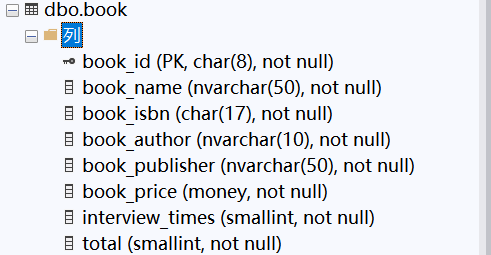
\includegraphics[width=0.7\textwidth]{img/add_total.png}
    \caption{添加total列结果}
\end{figure}

\subsubsection{3.2 修改interview\_times列数据类型为int}

\begin{lstlisting}[language=SQL]
ALTER TABLE book ALTER COLUMN interview_times int NOT NULL;
\end{lstlisting}

\begin{figure}[H]
    \centering
    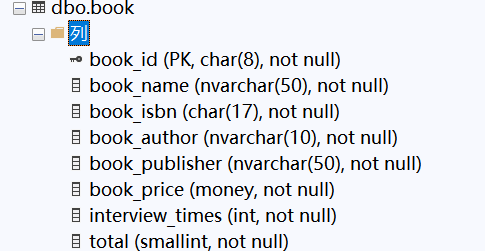
\includegraphics[width=0.7\textwidth]{img/modify_interview_times.png}
    \caption{修改interview\_times列类型结果}
\end{figure}

\subsubsection{3.3 删除total列}

\begin{lstlisting}[language=SQL]
ALTER TABLE book DROP COLUMN total;
\end{lstlisting}

\begin{figure}[H]
    \centering
    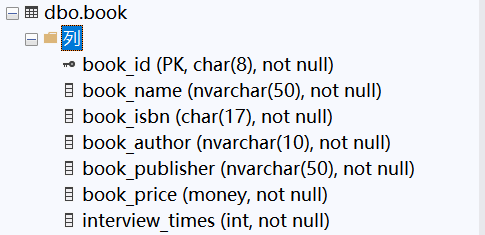
\includegraphics[width=0.7\textwidth]{img/delete_total.png}
    \caption{删除total列结果}
\end{figure}

\subsection{实验总结与易错点注意}

本次实验主要围绕数据库的定义与基本操作展开，包括数据库的创建、数据表的详细设计与实现，以及表结构的动态修改。通过实际操作SQL DDL语句，进一步理解了数据库对象的约束设置、字段类型选择和表结构变更的规范流程。实验提升了我对数据库系统原理的直观理解和动手能力。注意：先约束后列，删列先删依赖。

\textbf{常用指令（5条够用的）：}

\begin{lstlisting}[language=SQL]
CREATE DATABASE JY;
CREATE TABLE t (id int PRIMARY KEY);
ALTER TABLE t ADD col int NOT NULL DEFAULT 0;
ALTER TABLE t ALTER COLUMN col int;
ALTER TABLE t DROP CONSTRAINT DF_name; DROP COLUMN col;
\end{lstlisting}

\textbf{易错点：}

\begin{itemize}
    \item 删列忘先删约束 → 5074
    \item 旧表加 NOT NULL 不给 DEFAULT → 515
\end{itemize}

\end{document}